\documentclass[a4paper]{article}

\usepackage[english]{babel}
\usepackage[utf8]{inputenc}
\usepackage{amsmath} % matricies and math notation
\usepackage{graphicx} %Check if still needed, have been using tikz in place
\usepackage[colorinlistoftodos]{todonotes}
\usepackage{xcolor} % note: there's also a color package instead of xcolor
\usepackage{verbatim} % For block comments
\usepackage{tikz} % allow the drawing of images
\usepackage{amssymb} %for math notation that is needed
\usepackage{physics}
\usepackage{float} % Fixing formatting
\usepackage{multicol} %to allow sections to have different column styles
\usepackage{mathtools}%for more formatting stuff
\usepackage{hyperref} % allows for hyperlinks as well as makes underscores in a URL not break the document



%more complex installs with file dependancies
%\usepackage[american]{circuitikzgit} % To draw digital logic circuits 
	% Wasn't Used, commented out in case it's needed later
% http://texdoc.net/texmf-dist/doc/latex/circuitikz/circuitikzmanual.pdf
% circuitikz install instructions https://github.com/circuitikz/circuitikz/wiki/Installation

\label{depreciateRemove} %things that should be removed in final version but might still be useful here
\usepackage[matrix,frame,arrow]{xypic}
\usepackage{qcircuit}
%https://github.com/CQuIC/qcircuit



\label{includes} %creates a label for easy navigation

%TODO


\begin{comment}
	See github repository for current issues and required changes
\end{comment}
%%%%%%%%%%%%%%%%%%%%%%%%%%%%%%%%%%%%%%%%%%
\label{customCommands}
\definecolor{mygray}{gray}{0.6} % Low priority, see if this can be acheived without this dependancy
\usetikzlibrary{arrows.meta} %this might be redundant
%\newcommand{\volt}[1]{${#1} V$} % shortcut to volt
%\newcommand{\ohms}[1]{${#1} \Omega$} % shortcut to ohms
\newcommand{\tabhere}{} % Currently commented Out
\newcommand{\tabhereB}[1]{{#1}} % Currently commented Out
%\newcommand{\tabhere}{$\>\>\>\>$ } % Bypasses some formatting issues %backup
%\newcommand{\tabhereB}[1]{$\>\>\>\>$ {#1}} % Bypasses some formatting issues %backup


%\begin{comment} % test circuit, not error free but draws well, fix in later revision
%\begin{circuitikz}
%\draw (0,0) to[R= $\Omega${1}, i=?, \volt{84}] (2,0) --
%(2,2) to[V=\volt{84}] (0,2)
%-- (0,0);
%\end{circuitikz}
%\end{comment}



%%%%%%%%%%%%%%%%%%%%%%%%%%%%%%%%%%%%%%%%%%
\title{A Brief Introduction to Quantum Computing from the Perspective of Ladder Logic\vspace{-0ex}}
\author{Jerry Kensler\vspace{-0ex}}
\date{\today\vspace{-0ex}}
\usepackage{titling}
\begin{document}
	
		\maketitle %this one command gave way more trouble than it should have in regards to spacing
		\let\originalnewpage\newpage \let\newpage\relax \let\newpage\originalnewpage
		\begin{center}		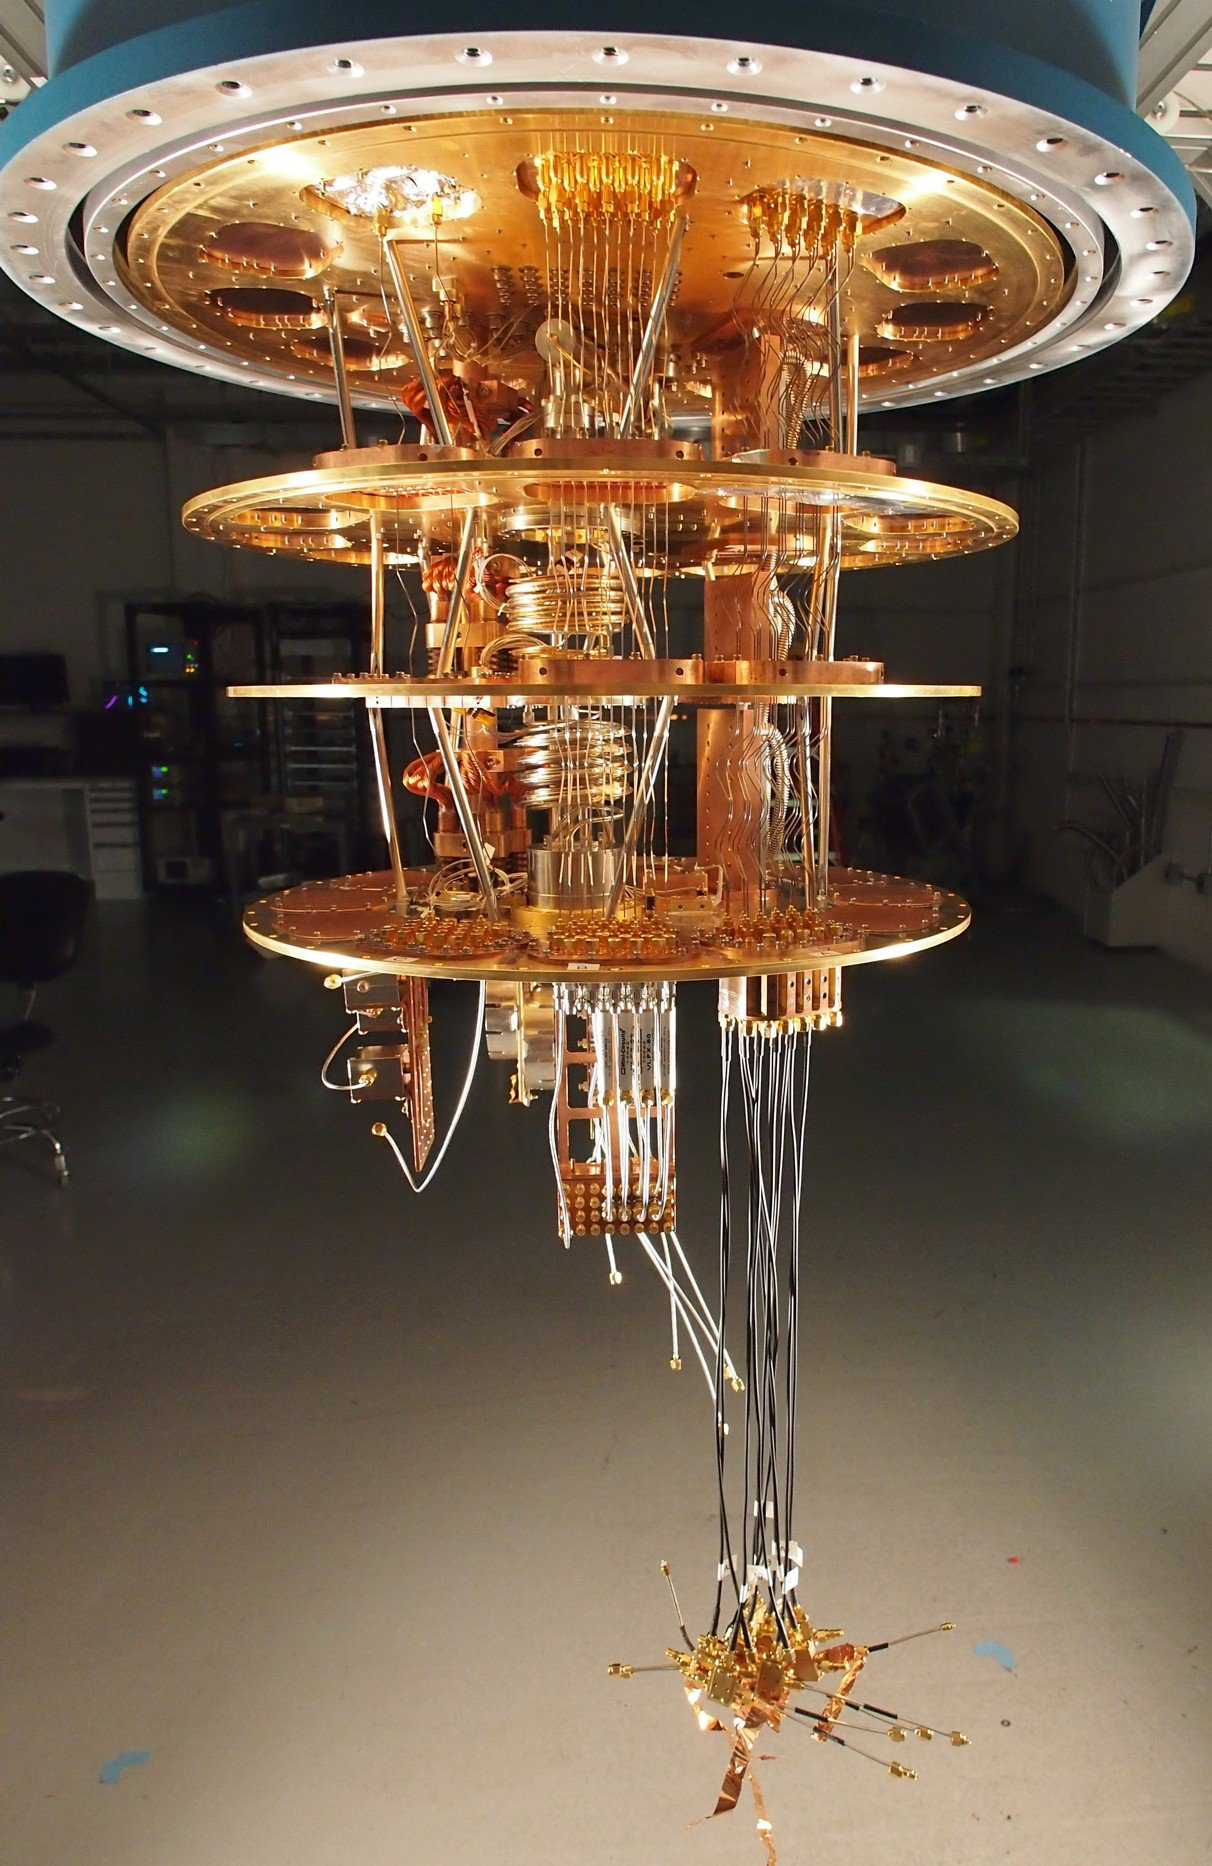
\includegraphics[scale=0.12]{googlequantumcomputer} % image source https://www.technologyreview.com/s/602283/googles-quantum-dream-may-be-just-around-the-corner/
		\end{center}
	\textcolor{mygray}{
			\begin{figure}%https://ai.google/research/pubs?area=QuantumAI
			\caption{Photograph of Bristlecone courtesy of Google\textcolor{red}{(CITE)}}\label{titleImage} %https://ai.googleblog.com/search/label/Quantum%20Computing
			%https://www.popsci.com/quantum-computer-photos  % Not the one needed
			\end{figure}}
	\begin{abstract}
		
		Quantum Computing is an advanced topic, it suffers from a perception of complexity beyond what is reasonable for the actual subject matter.  The intent of this paper is to soften that perception and bring the topic down to a less intimidating level.  The primary targets of this paper are students currently enrolled in or freshly graduated from an electrical engineering program; however, any individual with a base knowledge in programming or digital logic should be able to gain some level of benefit. 
		
		Keywords:  Quantum, QISKit, Computing, Ladder, Logic, QASM, Introduction
		% Author note: the intention of this paper is to fill some of the skill gap many novices encounter in learning quantum computing.  By no means should this be considered an all-encompassing guide to the subject matter.
	\end{abstract}
\newpage
%\raggedleft
%\setlength{\parindent}{15cm}
%\phantom{This text will be invisible, use it for search terms in different documents}
\section{Introduction}
\label{sec:introduction} % reword pass 1
%$\>\>\>\>$ tab should be 8? spaces
\tabhere Quantum physics as a whole is an exceptionally advanced topic and the applications, occasionally breaching into concepts such as particles that are both matter and antimatter\cite{mindBoggle} which may at first seem contradictory by their very nature.  Add to this many common misleading analogies and the fact that "Qubit" may refer to any number of technologies, such as ion traps, superconducting qubits, or spin qubits and it is no wonder that people get confused.  While quantum computing does use the underlying principles of quantum mechanics, it is still nothing more than a programming architecture.  To put this statement in another context, an individual does not need to understand how to bias a transistor to be good at programming in C.

\subsection{Use Case for Quantum Computing}% reword pass 1
\tabhere Quantum computing is a Disruptive Emergent Technology, meaning, as far as industry is concerned, the implementation of these concepts have not only never been seen in any technology prior, but they also have the potential to revolutionize how things are done should these implementations prove successful.  Quantum computing is not a magic bullet that can handle every problem; however, it does have the potential to be exceptionally good at problems that current technology has difficulty solving.  Examples of such problems can be as varied as weather prediction, mathematical factoring \cite{shorsAlgorithm}, and even protein folding \cite{dwavepfold}. 

\subsection{Relevance} %AKA, why should you care % reword pass 1
\tabhere %To avoid mincing words or dancing around the point, all that is fine, but this leads to the famous words (paraphrased ,of course) uttered at one point by nearly every person between the ages of twelve and nineteen: "Why should I care?".  To that, there are two primary categories of answers.  %redundant
First, advances in technology generally creates a higher standard of living, in the case of quantum computing, these advances may assist in finding the cure to debilitating diseases, reducing cost of living \textcolor{red}{(CITE OR REPLACE)}, or even allowing for a faster, more secure means to transport data (Quantum Internet \cite{qinternetNature}).  \newline 

Second is economics, the reality of the situation is that there aren't enough people who are skilled in this area to fit the demand.  Meaning, not only are jobs available to those with the skills to fill the required roles, but due to the shortage of supply when compared to the demand, these jobs generally pay quite well.  \cite{qc5ycommercialize}
\label{AddMoreDetailHere}

\section{Background Concepts} % Wording Pass 1
\label{sec:backgroundconcepts}
%brief intro to this section, needs rewording
%This section is not meant to be an exhaustive list, but, in my personal experience, learning about the background concepts below will greatly assist a person’s ability to better understand quantum computing.  The following sections will provide a brief explanation of the concepts.
This paper assumes the reader has some basic knowledge of programming and electronics.  The content will primarily focus on the act of programming itself as well as the topics needed to get to that point.  There are many topics which should be covered if one wishes to become skilled in quantum computing, most of which the reader will need to research independently; however, the sections below should provide enough context in order to provide a suitable starting point.


\subsection{Removing Misleading Assumptions} % Wording Pass 1
The first and easily one of the most important concepts in quantum computing is to understand that the general public and most media 'experts' do not work in the field of quantum computing.  Therefore, it is important to note that many of the common assumptions can be misleading or plain wrong due to lack of context or the background knowledge required to properly articulate the concepts at hand.\newline
\newline
One prime example of this is Erwin Schrödinger and the concept of Schrödinger's cat.  To preface, this is not at all meant to downplay or discredit his work, merely to illustrate that without proper context even an otherwise correct statement from a Nobel laureate can be misconstrued.  \newline
\newline %helpful link to brush up https://en.wikipedia.org/wiki/Copenhagen_interpretation
To briefly summarize, Schrödinger's cat is a brilliant thought experiment meant to illustrate a potential paradox present within the Copenhagen interpretation of quantum mechanics.  This thought experiment was meant to highlight the bizarre nature of EPR (Einstein, Podolsky, Rosen), or superposition states.  This is demonstrated via a cat, radioactive particle, flask of poison, and a Geiger counter being sealed in a theoretical box.  Should the counter detect radioactivity, the flask would be broken causing the cat to die immediately.  Under the Copenhagen interpretation of quantum mechanics, this cat should be considered simultaneously both alive and dead, however, looking into the sealed box will reveal either a very scared cat, or a testament to animals killed in the name of science. \newline
\newline
In context, this is meant to demonstrate the concepts of complex, superimposed states collapsing upon measurement. For better or worse, this concept of a not dead, yet dead cat in a box has spread like wildfire, it has become the cornerstone of what the public sees as quantum computing. This has allowed the idea that the quantum state is both 1 and 0 to become the very first thing that anyone learns in regards to quantum computing.  While this statement is not technically wrong, it is fundamentally incomplete. In many ways, it's similar to the question "which came first: the chicken, or the egg?", the answer to which can only be something along the lines of 'invalid question', as it not only fails to define what denotes the term chicken, but it also leads the individual being asked to assume the term 'egg' is specifically in the context of a chicken egg. \newline
 \newline
In reality, a better way to think of this is through vectors and complex numbers.  The value is in fact both 1 and 0, but it's that way not because it is two things in a binary sense, but because it is a complex mixing of both.  To put this back into cat analogies, let's take the premise back to the start.  There is a cat, that cat is now infected with a zombie pathogen.  For all purposes, the cat is neither alive, nor dead, as it cannot cleanly fit into either category, yet it does have many of the defining characteristics that comprise both.  From here, the cat is injected with an antidote,  being a rushed marvel of medicine meant to save the feline race, it will near instantly result in either a complete cure or certain death for our kitten subject.  For this analogy, the zombified state represents the ability of qubits to be in a mixed state, the antidote representing the act of measuring this mixed state and thus collapsing it into a binary value. %: 1 or 0, alive or dead.


\subsection{Balanced Ternary} %The basics from the ground up
%note: blanaced ternary is not, strictly speaking a core mechanic in quantum computing.  However, it could serve as a gentle introduction to non-binary coding for many students.  A bridge between hard digital and the strangeness of qubits

Balanced Ternary is not, strictly speaking a part of quantum computing, so with that knowledge, it may seem like a strange item to include as background information when discussing the subject. However, given this author's personal experience, it is nearly ideal to serve not only as a bridge to more advanced concepts but also as a demonstration of why said concepts are important. \newline
\newline
To do this, a brief nod to what numbers are at their core is needed. It's pretty obvious to most, but numbers are nothing more or less than a way to categorize quantity.  This concept of quantity is important as it is independent of stylistic choices such as base or notation.  In programming, binary is frequently used as it reflects the power state of transistors within the register.  For most general cases, this works quite well allowing for any number of tricks, or bit-hacks, to be employed to speed things up.  However, unsigned binary does have an Achilles' heel in that due to its basis in positive numbers, there is no simple way to show when a number is negative on hardware \footnote{Note: the "-" symbol seen in both binary and standard decimal is not a representation of quantity, it's more akin to a shorthand for the operation of 0 - Quantity, and thus it's fairly difficult to represent in hardware}.  To do so, one needs to employ a tactic such as the IEEE 754 standard, adding much more complexity than would otherwise be necessary.  One way to circumvent this issue is to use a balanced number system such as balanced ternary. \newline
\newline
These systems work by designating symbols as pre-signed.  In the case of balanced ternary, the symbols are designated as "0; +; -" and they represent "$3^{(s*n)}$" with "n" being the index number starting at zero from right to left and "s" being the sign as denoted by the "+" for positive, "-" for negative, or "0" for null quantity \footnote{ This notion of sign polarity being a property of quantity will become relevant in later sections (~\ref{ternaryRelevance}), but for now, it is acceptable to use this idea as a base case.}.  From there it is a simple matter of adding the positive and negative values up in order to get the end result (see Table~\ref{tab:ternary}, for example and comparison between bases).

\begin{table} %Table used to illustrate comparison between bases
	\centering
	\begin{tabular}{l|l|l} % Justification l-left, c-center, r-right
		Signed Decimal & Binary (IEEE 754*) & Balanced Ternary \\\hline %might remove the 754 example if it becomes an issue to clarity
		0 & 0 & 0 \\
		3 & 11 & 10 \\
		5 & 101 & + 0 - \\
		-254 & 11000011011111100000000000000000* & - 0 0 - + - \\ % -3^5 + 0 + 0 - 3^2 + 3^1 -3^0
	\end{tabular}
	\caption{\label{tab:ternary}Comparison table showing equivalent numbers in different display forms}
\end{table}
\subsection{Vectors \textcolor{red}{(Explain Each New symbol)}}
\label{THISNEEDSACCURACYREVIEW} % Getting into nitpick notation stuff, need to be careful
A proper discussion of quantum computing cannot be had without discussing vectors and their function in understanding the circuit.  This will be discussed more in a later section (\ref{Qubits}); however, the shorthand version is as follows.  Due to the fact that quantum computers operate on qubits rather than classical (binary) bits, a quantum computer is effectively nothing more than a very complex probabilistic vector equation. To be specific, this state space $\mathcal{H}$, is not just vector space but a Hilbert space, meaning it has a positive-definite Hermitian inner product $\bra{\cdot}\ket{\cdot}$.  This has quite a few implications and entire papers can be written on the vector space alone, but in simple terms what it means is that the sum of the probabilities of a quantum computer being in any given state post measurement will always be 1.

\subsubsection{Notation}
%https://tex.stackexchange.com/questions/214728/braket-notation-in-latex
In quantum computing, and quantum mechanics as a whole for that matter the standard notation is Bra-Ket notation, also known as Dirac notation. Example: $\bra{\phi}\ket{\psi}$. The right part, called ket, is typically represented as a column vector and written as $\ket{\psi}$. The left part, called bra, is the Hermitian conjugate of the ket with the same label, is typically represented as a row vector and written as $\bra{\phi}$. \newline
\newline
This may seem like a bit much for those whom have never worked with this sort of thing before, but the following example should help clarify things.\newline
$\ket{\psi}=\alpha\ket{H} + \beta\ket{V}$ \newline
What the above example notates is the simplest meaningful version of a quantum system that can be in two possible states, for example the polarization of a photon. When measured, the system will collapse into either the horizontal state $\ket{H}$ or the vertical state $\ket{V}$, until that moment it exists in a superposition of the two.  To find the probability of the system collapsing into a given state upon measurement, simply take the multiplier in front of the desired ket and square it.  For instance, in the case of finding the probability of a vertical state the answer would be $\beta^2$. \newline
\newline
Back to the previous section, the fact that the sum of the probability of all possible states is equal to 1 was brought up.  This can be notated as:\newline
$\sum\psi^{*}_{n} \psi_{n}=1$ \newline
This will be discussed in more detail in the qubit section (\ref{Qubits}) in regards to what are called bloch spheres. % don't go too deep into superposition yet

%$\expval{A}{\Psi}$

%http://detexify.kirelabs.org/classify.html
%Use to help figure out what symbol is where and how to write it out

\section{Advanced Concepts}
\label{sec:AdvConcepts}
The following sections are more advanced concepts moving towards the target goal of quantum circuits.  These sections assume that the reader understands all prior sections and has completed further reading when necessary. 


%helpful link: https://arxiv.org/pdf/quant-ph/0406003.pdf Q-circuit latex tutorial
% https://www.media.mit.edu/quanta/qasm2circ/
%https://github.com/CQuIC/qcircuit Qcircuit package location
%https://tex.stackexchange.com/questions/32839/drawing-circuit-diagrams-with-logic-gates-in-latex
%self note: tons of comments here


\begin{comment} % A helpful Demo circuit graphic, delete dependancy and this once it is removed in favor of using tikzpicture
\begin{circuitikz} 
	\draw
(0,2) node[and port] (myand1) {}
(0,0) node[and port] (myand2) {}
(2,1) node[xnor port] (myxnor) {}
(myand1.out) -- (myxnor.in 1)
(myand2.out) -- (myxnor.in 2);
\end{circuitikz}
\end{comment}

\subsection{Reversible Logic Gates} %The basics from the ground up
%there was a time when reversible logic was seen as a fatal flaw in QC, but some dude who was pretty clever figured out any standard logic gate could be simulated within reversible logic
A more advanced concept that is still core to quantum computing is the idea of reversible logic gates. Normally when it comes to digital logic inputs and outputs are decoupled. Consider the digital logic circuit as seen in Figure~\ref{Circuit:1}.  In this circuit, there are three inputs and a single output, even knowing the gate layout and the end value of $f_{1}$, the best that could be done for determining the input values is narrowing it to a range of possibilities as all the values have been combined into one, irreversible output. Now consider the reversible logic circuit as seen in Figure~\ref{Circuit:2}, while the notation may be unfamiliar\footnote{This notation is that of a simple quantum ladder logic circuit, the elements of which will be covered in section~\ref{QladderLogicHere}}, each input has its own unique output.  Due to this, so long as one knows what gates are in the circuit and what the output values are, the input values can be derived relatively easily.

%consider deleting circuitikz if it isn't used elsewhere


\begin{figure}[H] %note: Tikz does not like playing with multiple circuits.  Either find a solution by learning the syntax well enough to compensate or don't use any more standard circuits.  Given that this paper isn't on standard digital circuits, the latter is likely the better option
%	\centering
\label{tikzSettings} %in case it needs to move up
\usetikzlibrary{arrows, shapes.gates.logic.US, calc}
\tikzstyle{branch}=[fill, shape=circle, minimum size=3pt, inner sep=0pt]
\begin{tikzpicture}
\node (x) at (0, 2) {$x_{1}$};
\node (y) at (0, 1) {$x_{2}$};
\node (z) at (0, 0) {$x_{3}$};

\node[not gate US, draw] at ($(x) + (0.8, 0)$) (notx) {};
\node[not gate US, draw] at ($(y) + (0.8, 0)$) (noty) {};
%\node[and gate US, draw, rotate=0, logic gate inputs=nnnn] at ($(noty) + (2, 0.085)$) (xory) {};
\node[or gate US, draw, rotate=0, logic gate inputs=nnn] at ($(noty) + (2, 0.085)$) (xory) {};

\draw (x) -- (notx.input);
\draw (y) -- (noty.input);

\path ($(notx.input) + (0.2, 0)$) -- coordinate (puntx) (x |- notx);
%\draw (x) -- (puntx) node[branch] {} |- ($(notx.output) + (0.4, 0.4)$) |- (xory.input 1);

\draw (notx.output) -- ([xshift=0.2cm]notx.output) |- (xory.input 1);
\draw (noty.output) -- ([xshift=0.2cm]noty.output) |- (xory.input 2);
\draw (z) -| ($(noty.output) + (0.2, -0.5)$) |- (xory.input 3);

\draw (xory.output) -- node[above]{$f_{1}= \bar x_{1} + \bar x_{2} + x_{3}$} ($(xory) + (3.5, 0)$);
%\draw (xory.output) -- node[above]{$\overline{x + \bar x + \bar y + z}$} ($(xory) + (3, 0)$);
\end{tikzpicture}
\caption{Digital Logic Circuit}\label{Circuit:1}
\end{figure}

%\begin{comment}%debugging

\begin{figure}
 %helpful for understanding the syntax https://github.com/CQuIC/qcircuit/blob/master/Qtutorial.tex


%\small \begin{verbatim} %verbatim displays the code itself instead of rendering it
\[\Qcircuit @C=1em @R=0.5em @!R { %rows and columns, pretty standard
	 \lstick{\psi} & \targ & \targ & \qw & \targ & \meter \\
	 \lstick{\psi} & \ctrl{-1} & \qw &\qw & \qw & \meter \\
	 \lstick{\psi} & \qw & \ctrl{-2} & \qw & \qw & \meter \\
	 \lstick{\psi} & \qw & \qw & \qw & \ctrl{-3} & \meter\\
}\]
%\end{verbatim}}
%&\lstick{\ket{\psi}}
	\caption{Reversible Logic Circuit}\label{Circuit:2}
\end{figure}

%\end{comment}%debugging
\subsection{PLC Ladder Logic \textcolor{red}{images and content required}}
\label{PLC_Here}
%Rockwell Automation?


\subsection{Probability Current\textcolor{red}{ (Placeholder)}} %this topic is a terrifying monster
\label{ternaryRelevance} %allows linking to this spot regardless of location
%https://archive.org/details/MagneticAmplifiers
% Further Reading: http://sparkbangbuzz.com/mag-amp/mag-amp.htm 

% and oh boy is it a heavy topic, helpful link for some wording: https://www.math.ucdavis.edu/~greg/intro.pdf

In the previous section involving balanced ternary it was mentioned that the concept of quantities innately having a sign polarity would be relevant later, this section is that aforementioned later. Fair warning, this section will get very math heavy. \newline
\newline
% Use music to help explain this.  
% The sum of probability amplitudes is akin to the sum of notes playing in a chorus.  All of them constructively and destructively interfere with each other to make the music that is heard by our ears


\label{FigureisThecommandYouAlwaysForget}%saved a lot of time putting this here
\label{captionIsTheOtherOne}
%refer to https://www.st-andrews.ac.uk/physics/quvis/simulations_html5/sims/ProbabilityCurrent/ProbabilityCurrent.html 
%for a comprehensive/interactive display

% a good bloch sphere to use as a reference point for own graphics https://www.google.com/imgres?imgurl=http%3A%2F%2Fwww.activecyber.net%2Fwp-content%2Fuploads%2F2016%2F05%2FSlide2-1024x576.jpg&imgrefurl=http%3A%2F%2Fwww.activecyber.net%2Frise-quantum-computers-current-state-cryptographic-affairs%2F&docid=WlC5Z0oQpIQMoM&tbnid=PgRi_YmNYCO0VM%3A&vet=10ahUKEwjwndO69rHbAhVCHTQIHUmgDVwQMwhMKA8wDw..i&w=1024&h=576&client=firefox-b-1&bih=727&biw=1536&q=probability%20current%20graph%20quantum%20computing&ved=0ahUKEwjwndO69rHbAhVCHTQIHUmgDVwQMwhMKA8wDw&iact=mrc&uact=8



\begin{figure} %note this area is not yet complete as the equations are a beast to input
	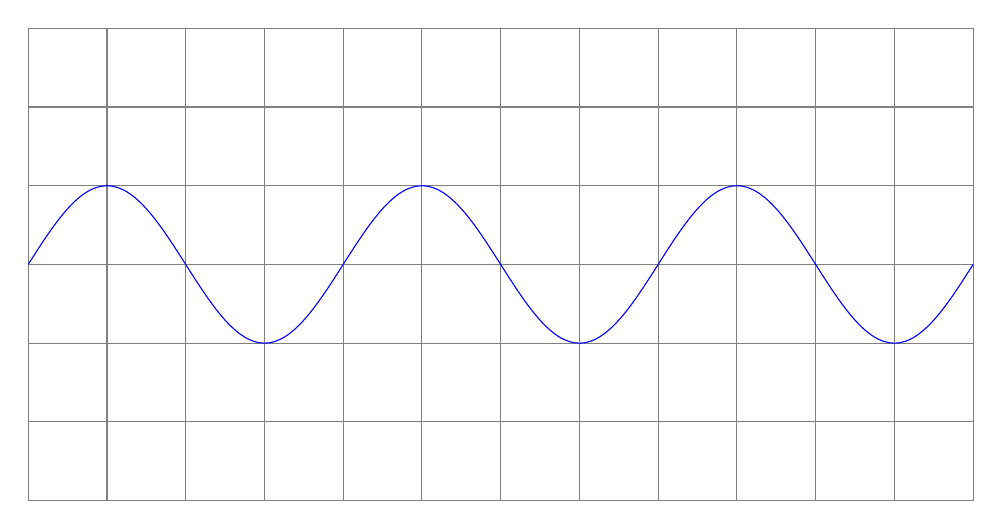
\begin{tikzpicture}
	\draw[gray] (0,-3) grid (12,3);
	%blue line start
	\draw[blue] (0,0) sin (1,1) cos (2,0) sin (3,-1) cos (4,0);
	\draw[blue] (4,0) sin (5,1) cos (6,0) sin (7,-1) cos (8,0);
	\draw[blue] (8,0) sin (9,1) cos (10,0) sin (11,-1) cos (12,0);
	%blue line end
	\end{tikzpicture}
	\caption{Probability Density Placeholder}\label{ProbDensity1}
\end{figure}


\begin{figure} %note: this area is not correct, you need two graphs, one for density and one for current
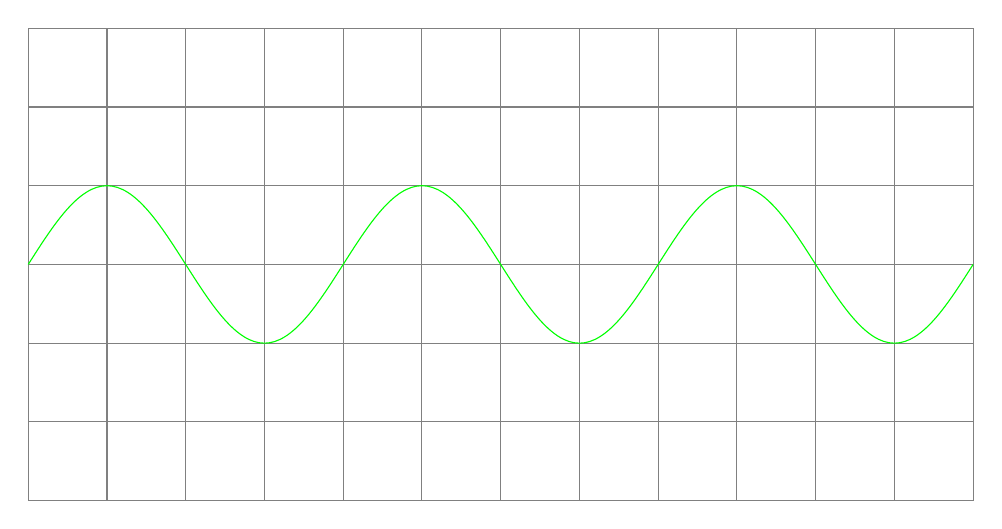
\begin{tikzpicture}
\draw[gray] (0,-3) grid (12,3);
%blue line start
\draw[green] (0,0) sin (1,1) cos (2,0) sin (3,-1) cos (4,0);
\draw[green] (4,0) sin (5,1) cos (6,0) sin (7,-1) cos (8,0);
\draw[green] (8,0) sin (9,1) cos (10,0) sin (11,-1) cos (12,0);
%blue line end
\end{tikzpicture}
\caption{Probability Current Placeholder}\label{ProbCurrent1}
\end{figure}


%\section{Hardware Implementation} %go over a few examples such as d-wave, topological, ion trap, josephson junctions and etc.  If a specific company pioneered or is the primary utilizer of an implementation, mention them by name
\newpage %should make it look better, remove if it becomes an issue

\section{Quantum Coding}
This section deals in the various coding languages utilized in programming quantum computers.  As these languages are still in active development, expect this section to change frequently.

\subsection{Quantum Ladder Logic}
\label{QladderLogicHere} %referenced in a previous section
%brief explanation of this stuff
\subsubsection{Qubits} %another section to check details heavily, might raise it up a level and move other things around
\label{Qubits}
Qubits are to quantum computers what register bits are to a classical computer. A qubit is a two-state quantum mechanical system based on properties such as photon polarization or the spin of a trapped ion.  

\paragraph{Decoherence} % could use a pass for wording, but a spinning top is a rather good analogy to explain entropy
In order to create the properties necessary to enable a quantum computer, specific conditions need to be met.  These conditions vary between machines but common threads among them include noise isolation and extremely low temperatures.  For IBM's machines these temperature can reach around 15 milli-Kelvin, a feat only capable with specialized hardware, and even then requiring several days to do so ~\cite{IBM_IsCold}. Due to this, and a myriad of other factors, qubits are inherently fragile, with stable states generally only lasting for periods of \textcolor{red}{CITE AND GRAB NUMBER} milliseconds. While this duration is constantly being improved upon by the tireless engineers and researchers across the many teams in quantum computing, to the programmer, the reality is that every operation counts. Much like a spinning top, a qubit (or set of qubits) has a finite amount of time before the system collapses into meaningless noise.  Keeping with the spinning top analogy, every operation performed on a given qubit is akin to a gentle nudge in order to guide its path.  Each nudge (or quantum gate) has a set cost in terms of run time with the more complex gates being akin to a large flick.  This is the process called decoherence, at its root, it is nothing more than entropy, but it must always be kept in mind when creating any quantum circuit.  


\paragraph{Bloch Sphere} %lots of nested sections in this area

See Figure~\ref{bloch1} for visual.  A Bloch sphere is a geometrical representation of the pure state space of a two level quantum mechanical system (qubit).\newline
\newline
Since the total probability of the system has to be one: $\bra{\psi}\ket{\psi}=1$ this gives us the constraint required in order to write $\ket{\psi}$  using the following representation. \newline
$\ket{\psi}=\cos(\dfrac{\theta}{2})\ket{0} + e^{i\phi}\sin(\dfrac{\theta}{2})\ket{1}=\cos(\dfrac{\theta}{2})\ket{0}+(cos(\phi)+i\sin(\phi))\sin(\dfrac{\theta}{2})\ket{1}$ \newline
Where $0\leq\theta\leq\pi$. \newline
\newline
All of that is a bit of a mouth-full, so to speak, but for most practical purposes, the Bloch sphere is one of the best tools to visually understand and debug a quantum circuit on the qubit level when it is an option that is available.

% Would be worthwhile to list how to find the X, Y, and Z components of the vector from a given sphere or visa versa
% See http://www.vcpc.univie.ac.at/~ian/hotlist/qc/talks/bloch-sphere-rotations.pdf
%for reference details

%further reading topic: Gyrovector Space


\begin{figure}%Draws a bloch sphere, make sure to label parts later
	%https://tex.stackexchange.com/questions/345420/how-to-draw-a-bloch-sphere
	
	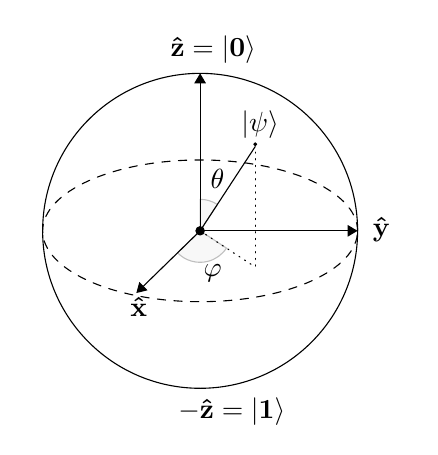
\begin{tikzpicture}[line cap=round, line join=round, >=Triangle]
	\clip(-2.19,-2.49) rectangle (2.66,2.58);
	\draw [shift={(0,0)}, lightgray, fill, fill opacity=0.1] (0,0) -- (56.7:0.4) arc (56.7:90.:0.4) -- cycle;
	\draw [shift={(0,0)}, lightgray, fill, fill opacity=0.1] (0,0) -- (-135.7:0.4) arc (-135.7:-33.2:0.4) -- cycle;
	\draw(0,0) circle (2cm);
	\draw [rotate around={0.:(0.,0.)},dash pattern=on 3pt off 3pt] (0,0) ellipse (2cm and 0.9cm);
	\draw (0,0)-- (0.70,1.07);
	\draw [->] (0,0) -- (0,2);
	\draw [->] (0,0) -- (-0.81,-0.79);
	\draw [->] (0,0) -- (2,0);
	\draw [dotted] (0.7,1)-- (0.7,-0.46);
	\draw [dotted] (0,0)-- (0.7,-0.46);
	\draw (-0.08,-0.3) node[anchor=north west] {$\varphi$};
	\draw (0.01,0.9) node[anchor=north west] {$\theta$};
	\draw (-1.01,-0.72) node[anchor=north west] {$\mathbf {\hat{x}}$};
	\draw (2.07,0.3) node[anchor=north west] {$\mathbf {\hat{y}}$};
	\draw (-0.5,2.6) node[anchor=north west] {$\mathbf {\hat{z}=|0\rangle}$};
	\draw (-0.4,-2) node[anchor=north west] {$-\mathbf {\hat{z}=|1\rangle}$};
	\draw (0.4,1.65) node[anchor=north west] {$|\psi\rangle$};
	\scriptsize
	\draw [fill] (0,0) circle (1.5pt);
	\draw [fill] (0.7,1.1) circle (0.5pt);
	\end{tikzpicture}
	
	
	\caption{Bloch Sphere}\label{bloch1}
\end{figure}

%\newpage %here for layout manipulation, comment out when not needed
\subsubsection{Circuit Layout} % Would Probably be helpful to have an introduction to how it actually worked prior to the meat


%\begin{figure}[H] %This keeps the code in the same place % note footnote doesn't play well with figure
	Similar to PLC Ladder logic (See section \ref{PLC_Here} for details),
	%\begin{multicols}{2} %multiple columns allows space to be better utilized for sections with circuits and the like
		\label{NEEDSMOAR} % and rewording
		 quantum circuits displayed in ladder logic generally follow a fairly well established layout. 		
		\[\Qcircuit @C=0.7em @R=0.5em @!R { %Spacing for rows and columns, pretty standard
			\lstick{Q_{1}=\ket{\psi}}& \qw	& \gate{!} & \qw	& \gate{?}	& \qw & \qw	& \meter \\	%& \cw \cwx \control{4}\\
			\lstick{Q_{2}=\ket{0}}& \qw	& \qw & \qw	& \gate{!}	& \qw & \qw	& \meter \\	%& \cw \cwx \control{4}\\
		}\]
	
	Unless otherwise noted, all quantum circuits are treated as going from left to right. Each row is a unique qubit and the line going across the row is the quantum wire \footnote{It is important to note here that all operations, including a 'blank' wire are 'gates' so to speak.  The implications of this will be discussed in the section regarding quantum gates (Section: \ref{QuantumGatesWhole})}.  In the above circuit, there are two qubits, the top qubit has been initialized to $\ket{\psi}$, or an arbitrary quantum state, below it the bottom qubit has been initialized to $\ket{0}$.  \newline
	\newline For theoretical purposes, most qubits in quantum circuits are notated as having an initial state of $\ket{\psi}$, this is to show that the algorithm these qubits are within works regardless of the input state of these qubits; however, when it comes to real-world applications, most qubits will start in a state of either $\ket{1}$ or $\ket{0}$ as it eliminates unnecessary variables when performing calculations. \newline
	\newline After initialization, the qubits continue along the wire from left to right in parallel.  Functionally, this is akin to having a vertical ruler with enough length to cover every row and a thin enough width to only take up a single column.  As this ruler advances, the operations under it will be evaluated. Any 'bare' wire will be evaluated as a no-op or no operation, and any gates will be evaluated for the time column they are contained in. \newline
	\newline In the case of our example circuit above, after the initial states are set, the order of operations is as follows~\footnote{For this example, the $\rightarrow$ symbol is being used to represent the advancement of time between columns/steps}:\newline \newline
	\fbox{$ Q_{1} = no-op; Q_{2}= no-op$}
	\fbox{$\rightarrow $}
	\fbox{$ Q_{1} = Gate "!"; Q_{2}= no-op$}
	\fbox{$\rightarrow $}
	\fbox{$ Q_{1} = no-op; Q_{2}= no-op$}
	\fbox{$\rightarrow $}
	\fbox{$ Q_{1} = Gate "?"; Q_{2}= Gate "!"$}
	\fbox{$\rightarrow $}
	\fbox{$ Q_{1} = no-op; Q_{2}= no-op$}
	\fbox{$\rightarrow $}\newline %otherwise it clips
	\fbox{$ Q_{1} = Measure; Q_{2}= Measure$}
	\newline \newline
	\label{CITENEEDEDHERE} % and wording adjustment
	This methodology of parallelism is a core property inherent to how a quantum computer processes data at a fundamental level. Thus, regardless of how a quantum computer is programmed, most quantum circuits can be approximated in this manor.
	

%\newpage


\subsubsection{Quantum Gates} %another mention of http://www.vcpc.univie.ac.at/~ian/hotlist/qc/talks/bloch-sphere-rotations.pdf
%turns out they have an exceptionally good explanation of Pauli gates
\label{QuantumGatesWhole}
Much like a digital logic gate operates on an individual or set of classical bits, a Quantum gate operates on individual or sets of qubits.  Given that each qubit is effectively a matrix, quantum gates are matrices which are used to modify the vector space. % Fact check, it's basically right, but after going on for a page about context and stuff, the last thing I want to do is be inaccurate.
\paragraph{Single-Qubit Gates}
%Pauli gates
\label{pauliGates} %this section is important

Among the single qubit gates, the most well known and frequently used are the Pauli gates, the Hadamard transform, the Phase gate, and the $\dfrac{\pi}{8}$ gate (denoted as T). These gates are as follows: \newline
\subparagraph{Pauli X} %this section has strange formatting, needs to be fixed later
\begin{multicols}{2}
\[\Qcircuit @C=1em @R=0.5em @!R { %rows and columns, pretty standard
	\lstick{ }   & \gate{X} & \qw \\
}\]
%\newline
	\begin{figure}[H]
		$\>$ \\ %this inserts a whitespace character so I can make a dummy line
		$\theta_{1}=\theta_{X} = \Bigg[\begin{matrix*}0&1\\1&0\end{matrix*}\Bigg]$
	\end{figure}
\end{multicols}





\subparagraph{Pauli Y}
\begin{multicols}{2}
\[\Qcircuit @C=1em @R=0.5em @!R { %rows and columns, pretty standard
	\lstick{ }  & \gate{Y} & \qw \\
}\]

	\begin{figure}[H]
		$\>$ \\ %this inserts a whitespace character so I can make a dummy line
		$\theta_{2}=\theta_{Y} = \Bigg[\begin{matrix*}0&-i\\i&0\end{matrix*}\Bigg]$
	\end{figure}

\end{multicols}


\subparagraph{Pauli Z}
\begin{multicols}{2}
\[\Qcircuit @C=1em @R=0.5em @!R { %rows and columns, pretty standard
	\lstick{ } & \gate{Z} & \qw \\
}\]

	\begin{figure}[H]
		$\>$ \\ %this inserts a whitespace character so I can make a dummy line
		$\theta_{3}=\theta_{Z} = \Bigg[\begin{matrix*}1&0\\0&-1\end{matrix*}\Bigg]$
	\end{figure}

\end{multicols}

\subparagraph{Hadamard Transform}
\begin{multicols}{2}
	\[\Qcircuit @C=1em @R=0.5em @!R { %rows and columns, pretty standard
		\lstick{ } & \gate{H} & \qw \\
	}\]
	
	\begin{figure}[H]
		$\>$ \\ %this inserts a whitespace character so I can make a dummy line
		$\theta_4 = \theta_H = \frac{1}{\sqrt{2}} \Bigg[\begin{matrix*}1&1\\1&-1\end{matrix*}\Bigg]$	% math matrix stuff	
	\end{figure}
	
\end{multicols}
\subparagraph{Phase Gate}
\begin{multicols}{2}
	\[\Qcircuit @C=1em @R=0.5em @!R { %rows and columns, pretty standard
		\lstick{ } & \gate{S} & \qw \\
	}\]
	
	\begin{figure}[H]
		$\>$ \\ %this inserts a whitespace character so I can make a dummy line
		$\theta_{5}=\theta_{S} = \Bigg[\begin{matrix*}1&0\\1&i\end{matrix*}\Bigg]$
	\end{figure}
	
\end{multicols}
\subparagraph{$\frac{\pi}{8}$ or T gate}
\begin{multicols}{2}
	\[\Qcircuit @C=1em @R=0.5em @!R { %rows and columns, pretty standard
		\lstick{ } & \gate{T} & \qw \\
	}\]
	
	\begin{figure}[H] %H is to designate "Here"
		$\>$ \\ %this inserts a whitespace character so I can make a dummy line
		$\theta_{6}=\theta_{T} = \Bigg[\begin{matrix*}1&0\\1&exp(\frac{i\pi}{4})\end{matrix*}\Bigg]$
	\end{figure}
	
\end{multicols}
\paragraph{Special Single-Qubit Gates}
The Following gates are special cases of the single qubit gates and thus deserve specific mention as thus.



\subparagraph{Measurement Gate}
% Extended Reading: 
% https://stackoverflow.com/questions/36262270/how-does-measurement-gate-work
% http://www-inst.eecs.berkeley.edu/~cs191/sp12/notes/chap1&2.pdf
% https://physics.stackexchange.com/questions/184524/what-is-the-difference-between-general-measurement-and-projective-measurement/184540#184540



	\[\Qcircuit @C=1em @R=0.5em @!R { %rows and columns, pretty standard
			\lstick{\ket{\psi}} & \meter &  \rstick{} \cw & \dstick{1 \> or \> 0} \\ %qwx %rstick %dstick 
	}\] \newline
	Even among special case quantum gates, the measurement gate stands out as unique.  Unlike all other quantum gates which take in a quantum state, and output a transform of that gate, the measurement gate takes in a quantum gate, then collapses it to output a binary value. As such it's one of the only non-reversible gates in quantum computing \textcolor{red}{CITE THIS}. \newline\newline
	In practice, while some circuits do measure mid run, it's impractical due to factors such as run time and decohesion, thus measurement gates are typically used at the end of a circuit in order to pass results to a digital computing device.
	


\paragraph{Multi-Qubit Gates} 
\label{advancedGates}
In addition to single qubit gates, most quantum circuits also utilize multi-qubit gates. There are many different types of these, but the most basic case is the controlled gate. 

\subparagraph{Control}

\begin{multicols}{2}
	\[\Qcircuit @C=1em @R=0.5em @!R { %rows and columns, pretty standard
		\lstick{ } & \ctrl{0} & \qw \\
	}\]
	
	%\begin{figure}[H]% H is not for Hadamard, it just puts the diagram "here"
	%	$\>$ \\ %this inserts a whitespace character so I can make a dummy line
	%	$\theta_4 = \theta_H = \frac{1}{\sqrt{2}} \Bigg[\begin{matrix*}1&1\\1&-1\end{matrix*}\Bigg]$	% math matrix stuff	
%	\end{figure}


\end{multicols} 

\subparagraph{Advanced Controls}

\begin{multicols}{2}
	\[\Qcircuit @C=1em @R=0.5em @!R { %rows and columns, pretty standard
		\lstick{ } & \ctrlo{0} & \qw \\
	}\]
	
	%\begin{figure}[H]% H is not for Hadamard, it just puts the diagram "here"
	%	$\>$ \\ %this inserts a whitespace character so I can make a dummy line
	%	$\theta_4 = \theta_H = \frac{1}{\sqrt{2}} \Bigg[\begin{matrix*}1&1\\1&-1\end{matrix*}\Bigg]$	% math matrix stuff	
	%	\end{figure}
	
	
\end{multicols} 











\begin{comment}% backup area
\begin{multicols}{2}
	\[\Qcircuit @C=1em @R=0.5em @!R { %rows and columns, pretty standard
		\lstick{ } & \gate{H} & \qw \\
	}\]
	
	\begin{figure}[H]% H is not for Hadamard, it just puts the diagram "here"
		$\>$ \\ %this inserts a whitespace character so I can make a dummy line
		$\theta_4 = \theta_H = \frac{1}{\sqrt{2}} \Bigg[\begin{matrix*}1&1\\1&-1\end{matrix*}\Bigg]$	% math matrix stuff	
	\end{figure}
\end{multicols} 
\end{comment}




\subsection{Quantum Assembly Language} % Open quantum assembly language: https://arxiv.org/abs/1707.03429
\label{currentSpot} %to find where I last left off
Quantum Assembly Language~\cite{qasmWhitePaper}, also known as QASM or OpenQASM is a coding back end that is widely used throughout industry.  It was developed to solve many of the coding issues that had been plaguing the architecture due to lack of a widely accepted standard.  As well as being part of IBM's Quantum Experience interface, its utilization can be seen in projects such as QISKit as well as many smaller projects. \newline
\newline
In terms of programming, QASM is relatively straightforward; there are only two types of storage, classical registers, and quantum registers.  These registers are nothing more than  one dimensional arrays of bits or qubits respectively and can then have gates applied to them which are unitary subroutines. Below is an example of QASM in use as well as the quantum ladder logic equivalent.

\begin{figure}[H] %This keeps the code in the same place
\begin{multicols}{2} %multiple columns allows space to be better utilized for sections with circuits and the like
\begin{verbatim}
include "qelib1.inc";

def c-Z,1,'Z'

qubit q0, $\psi$
qubit q1, 0
qubit q2, 0

H q1
cnot q0,q1
cnot q1,q2
cnot q0,q1
cnot q1,q2
H q0
c-Z q2,q0
H q0
H q0

measure q[0] -> c[0];
measure q[1] -> c[1];
measure q[2] -> c[2];
\end{verbatim}

Which Equates to the following code in Ladder Logic
\[\Qcircuit @C=0.7em @R=0.5em @!R { %Spacing for rows and columns, pretty standard
\lstick{\ket{q_{0}}=\ket{\psi}}& \qw		& \ctrl{1} 	& \qw 			& \ctrl{1}		& \gate{H}	& \gate{Z}	&\gate{H}&\gate{H}	& \meter \\	%& \cw \cwx \control{4}\\
\lstick{\ket{q_{1}}=\ket{0}} 	& \gate{H} 	& \targ 	& \ctrl{1}		& \targ 		& \ctrl{1}	& \qw 		&\qw & \qw	& \meter \\	%& \cw \cwx \control{3}\\
\lstick{\ket{q_{2}}=\ket{0}} 	& \qw 		& \qw 		& \targ 		& \qw 			& \targ 	& \ctrl{-2}	&\qw & \qw		& \meter  \\ %
}\]
\end{multicols} %and go back to normal formatting
\end{figure}
The circuit and code given above is for a known simplification of quantum teleportation~\cite{nielsonChuangQCQI}.   \textcolor{red}{(Repeated Content?)}



\section{Experiment \textcolor{red}{(Provide screencaps for each)}} 
This section contains information on experiments performed on both real world quantum computers as well as simulations and approximations of quantum computers.

%discuss pros and cons of each system, language, interface etc.

\subsection{IBM Quantum Experience}
%basic sum of it
When this project first began, IBM's Quantum Experience (IBMQE) was still very young.  It was and still is revolutionary in that it gave registered users the ability to program and test code on real quantum computers.  The next sections will cover details in regards to the primary methods of programming through this interface.
\subsubsection{Ladder logic} % cite sources for JJ stuff
For most users of IBMQE this is the primary thing they'll see.  It's a standard ladder logic interface and because of this, it is fairly intuitive.  With that said, because IBMQE is running on real hardware, it suffers from the restrictions of said hardware.  Qubits here are implemented physically via Pi Josephson Junctions, effectively a superconducting anharmonic oscillator.  This means that the frequency a qubit is oscillating at determines what qubits it can interact with.  Speaking from experience, to a new user that is extremely confusing if one isn't given an explanation.  The interface also lacks many basic multi-qubit gates due to their physical implementation not being possible at current time.\newline
\newline
IBMQE can move into a pure simulation mode, but it lacks the live feedback to properly make that mode seem responsive.  Where it does excel is in the next section, Quantum Assembly language (QASM).
\subsubsection{QASM} %redo wording
In addition to the ability to program in ladder logic, IBMQE allows users to code their circuits in QASM.  This feature is extremely powerful as users can not only code in ladder logic or QASM, but they can also flip between them depending on what view best suits their needs.  A skilled user can easily define custom gates based on matrices should the standard pauli gates not be sufficient.  

%\subsubsection{Limitations} % Reserve, should be covered pretty well in previous sections
%\subsection{QISKit}%API called from external code
\label{QISKit}
%While this section is currently commented out, it is quite important to include in later versions of this document

%basic summary: QISKit is an api that allows classical programming languages such as python to communicate with quantum computers
%Real world Implementations: Quantum Battleship, Using game to determine efficiency

\subsection{Quirk}%Easily one of the best interfaces
\subsubsection{Definition} % Changed from "What it is"
Quirk is an idealized, online drag-and-drop quantum circuit simulator. This simulator is hosted on Craig Gidney's block Algorithmic Assertions\cite{algoassert}.  It is open source and due to the fact that he works as a part of Google's Quantum AI Team, it is owned by Google.
\subsubsection{Pros}%make better name
Among all currently available quantum simulation interfaces, this one stands out from the crowd.  It is responsive, accessible online without having to download software and extremely intuitive.  All in all, it's an excellent place to begin learning about quantum computing, especially given that the blog hosting it has a plethora of articles about the inner workings of many quantum algorithms.
\subsubsection{Cons}%Also needs a better name
For all the Quirk interface brings to the table, there is one very important thing that it does not do.  Quirk is incapable of interfacing with a live quantum computer via API or otherwise; moreover, given the fact that circuits are stored as URL's to be generated, this severely limits how well the code can store as all it takes to lose a code is accidentally overwriting the clipboard or text document that said circuit is stored within.

\textcolor{red}{(Create a table comparing the various simulation and programming interfaces)} % Possibly similar to something like GSM arena except instead of comparing phones, compare quantum giblets

\section{Results and Interpretation}% 2-3 pages

\subsection{Example Source Code}
The following are examples of code that was run live on a quantum computer, specifically on IBM Q 5 Yorktown and related devices. 
\subsubsection{Superdense Coding}
In this section, the code provided is in both QASM and ladder logic.  It is worth noting that there is a discrepancy between the ladder logic and the QASM in regards to the cnot and controlled z gates.  This is due to the fact that at this time, there is no direct hardware implementation of a controlled z gate, thus for simplicity's sake the QASM code assumes non-existent control bits of 1.  This assumption can be changed to a control bit of zero by commenting out these gates. See Figure~\ref{IBMQE:ExampleResuts} in the Appendix for an example of program output on IBM's interface.

%\begin{small}

\begin{multicols}{2}
\begin{verbatim}
include "qelib1.inc";
qreg q[5];
creg c[5];
h q[0];
cx q[0],q[1];
x q[0];
z q[0];
cx q[0],q[1];
h q[0];

measure q[0] -> c[0];
measure q[1] -> c[1];
\end{verbatim}
%\end{small}
Which Equates to the following code in Ladder Logic
\[\Qcircuit @C=1em @R=0.5em @!R { %rows and columns, pretty standard
	\lstick{0} 		& \gate{H}	& \ctrl{1} 	& \gate{X} 	& \gate{Z}		& \ctrl{1}		& \gate{H}		& \meter \\	%& \cw \cwx \control{4}\\
	\lstick{0} 		& \qw 		& \targ 	& \qw 		& \qw 			& \targ			& \qw 			& \meter \\	%& \cw \cwx \control{3}\\
	\lstick{\psi} 	& \qw 		& \qw 		& \ctrl{-2}	\\ %line done
	\lstick{\psi}	& \qw 		& \qw 		& \qw 		& \ctrl{-3}		\\ %line done
	%\lstick{\psi} \\%	& \qw 		& \qw 		& \qw 		& \qw			& \qw 			& \qw 			& \qw 		& \meter  \\
	%\lstick{C}		& \qw 		& \qw 		& \qw 		& \qw			& \qw 			& \qw 			& \qw 		& \meter  \\
}\]



\begin{comment}%decided against image, kept here in case I reverted back again
\begin{figure}
	\begin{center}
		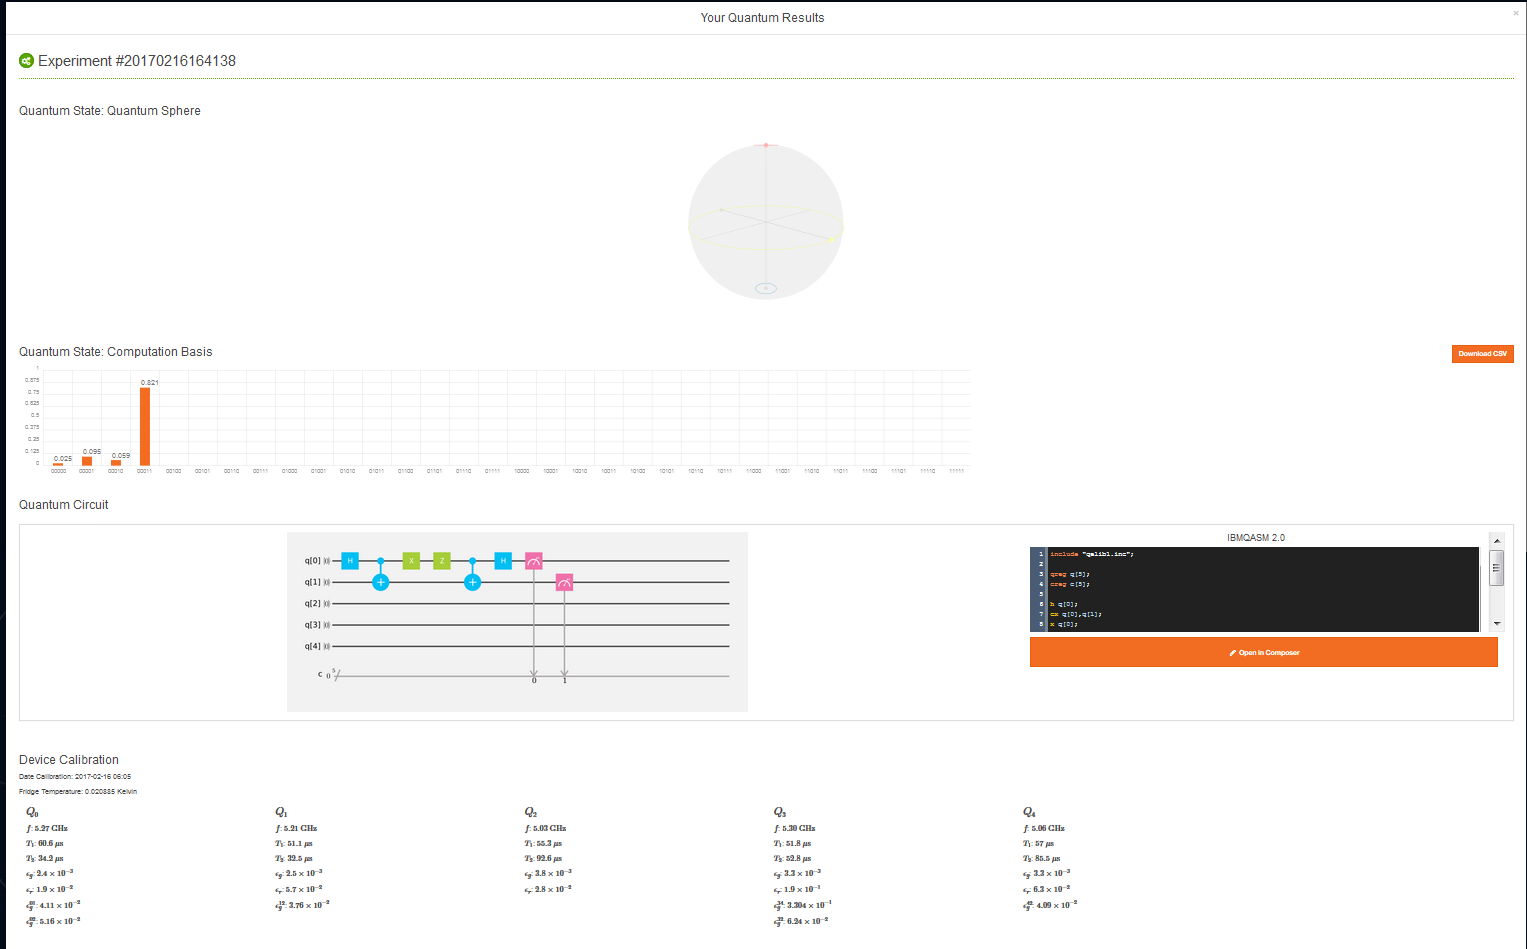
\includegraphics[scale=0.34]{ScreencapIBMQE_Superdense} 
	\end{center}
	\caption{Example IBM Quantum Experience Results}\label{IBMQE:ExampleResuts}
\end{figure}
\end{comment}
\end{multicols}
This may not seem like much at first glance but this small circuit shows many of the key fundamentals of quantum computing.  Within this small circuit are important concepts such as superposition, entanglement, and even advanced controls.  These all coalesce to enable the top qubit to carry two bits of information which are controlled by the bottom two gates. From there, it can be referenced to the qubit that was previously entangled with it in order to determine what the net change is and output the results via measurement.

\subsection{Analysis \textcolor{red}{(Provide list of original goals)}} %First person should be fine for this section given that it's commentary
Given that the goal of this project was to teach myself the basics of quantum computing and provide a path for other undergraduates to do the same, this project was a resounding success.  In the scope of this project, I taught myself the following languages: Quantum Ladder Logic, Quantum Assembly Language, Q\# (Microsoft's Quantum Computing language), LaTeX, CSS, and how to work with QISKit a specific coding API for quantum computers which is written in Python.\newline
\newline
In addition to the coding languages this project enabled me to pursue, I was able to meet with multiple professionals in the industry of Quantum Computing, from PhD's in quantum physics, to up and coming startups. \textcolor{red}{(Nod to companies and people perspectives, do not give individual's names)}  Moreover, the knowledge and source material required for this project to happen has also been requested by multiple professors at varied levels of teaching.  Partly in response to this, I have set up this paper to be hosted on GitHub so that anyone can provide feedback, allowing this document to stay relevant.

\subsection{Future Plans}
For future plans, this project is something I intend to continuously work on, with the eventual goal of including in depth tutorials for all extant programming languages in quantum computing.  At this point it has already been multiple years since this project was originally started and in all likelihood, this will be maintained and improved for years to come. It would be beneficial to add a few industry professionals to oversee the document, ensuring accuracy by catching errors that I would not notice.  Additionally, in time it should be possible to incorporate more features into this paper whether via source code or the output PDF itself, separating out functions such as the Bloch sphere into its own library that anyone would be able to use.




%\section{Discussion} % 1/2 page to a page, %bring this section back from commenting if it is deemed nessisary

%%%%%%%%%%%%%%%%%%%%%%%%%%%%%%%%%%%%%%%%%%%%%%%%%%%%%%%%%%%%%%%%%%%%%%%

%Beyond this point is mostly biblio and other resources such as images

%%%%%%%%%%%%%%%%%%%%%%%%%%%%%%%%%%%%%%%%%%%%%%%%%%%%%%%%%%%%%%%%%%%%%%%
\newpage
\section{Appendix} %Might need a different name, for larger images that don't fit in elsewhere
%not sure if there's a fix for the strange image placement that tex does

\begin{figure}[H] % Display image under the section name
\begin{center}
	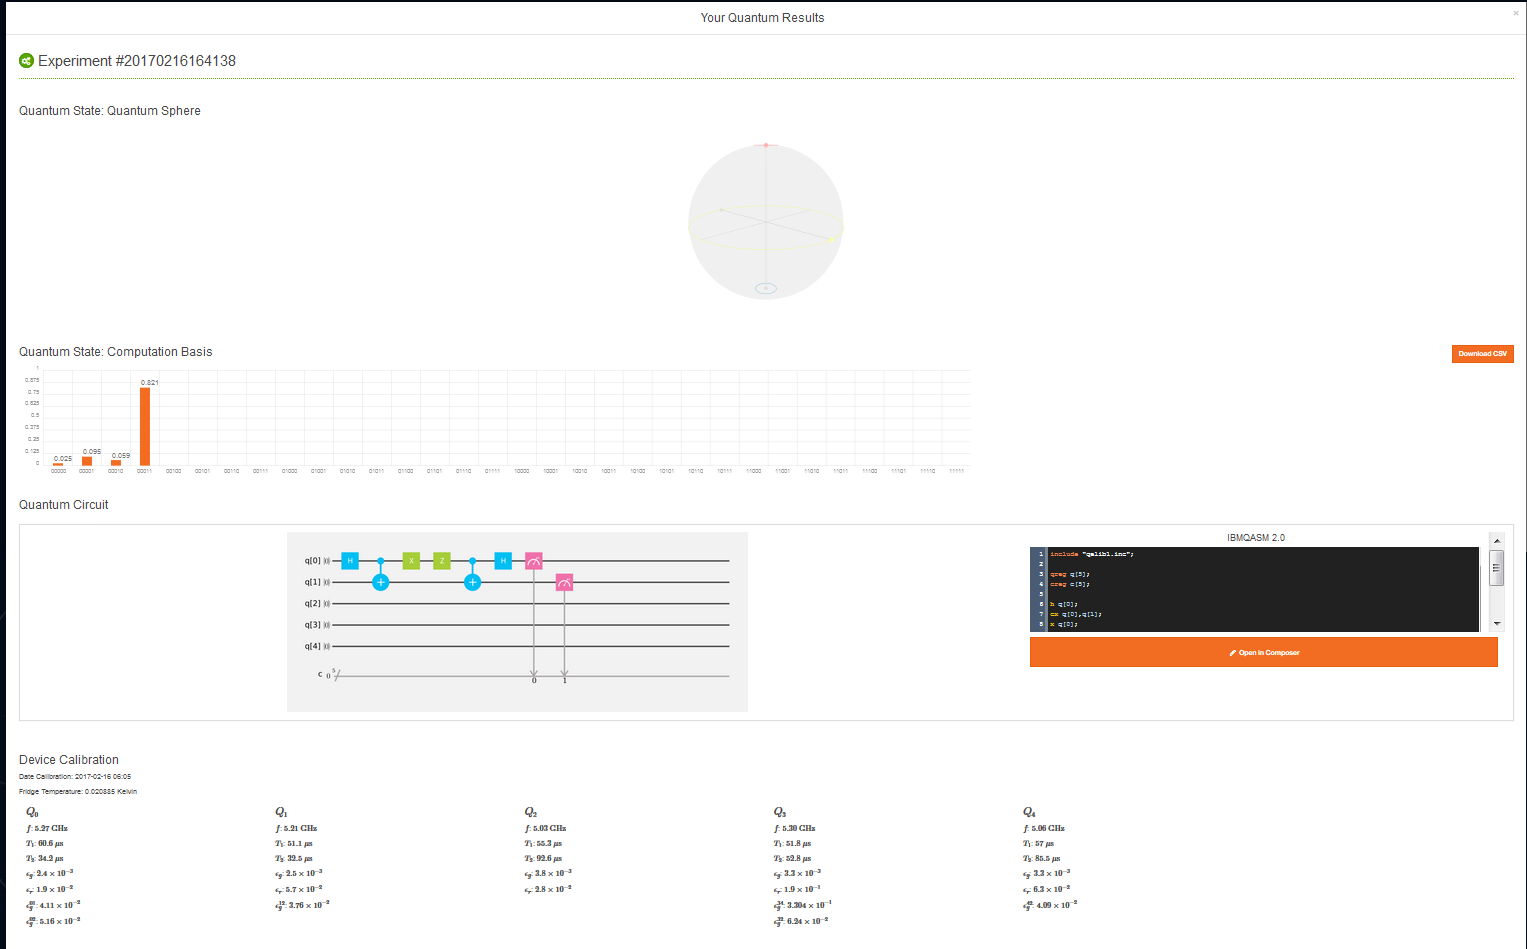
\includegraphics[scale=0.34]{ScreencapIBMQE_Superdense} % image source https://www.technologyreview.com/s/602283/googles-quantum-dream-may-be-just-around-the-corner/
\end{center}
\caption{Example IBM Quantum Experience Results}\label{IBMQE:ExampleResuts}
\end{figure}


%%%%%%%%%%%%%%%%%%%%%%%%%%%%%%%%%%%%%%%%%%%%%%%%%%%%%%%%%%%%%%%%%%
\newpage
\begin{comment}
\section{Bibliography}
\end{comment}%this is used to trick the navigation side bar into thinking there is a dedicated bibliography section without messing with the formatting as the block comment isn't recognized as comment until after the sections render on sidebar


\begin{thebibliography}{9}
	\label{sec:bibliography} %allows for quick navigation via side bar	
%========================================================================================

%\bibitem{template}
%	AuthorLast, AuthorF MI. \emph{"TitleOfSource.} OptionalCityOfPublication, OptionalDateOfOriginalPublication" TitleOfContainer. Version, OtherContributers, NumberSuchAsEpisodeVolume. Publisher, PublicationDate, LocationSuchAsPageNumberOrURL_Or_DOI. AccessedDayMonthSpelledOutYear

%https://owl.english.purdue.edu/owl/resource/747/01/


%from: https://en.wikibooks.org/wiki/LaTeX/Hyperlinks
%\url{<my_url>}
%\href{<my_url>}{<description>}
%mailto:my_address@wikibooks.org}{my\_address@wikibooks.org}
%========================================================================================
% Something to keep an eye on: https://github.com/strangeworks 
\bibitem{IBM_IsCold} % this link actually broke the entire document at one point due to underscores
	IBM Research, IBM QX Team. \emph{"The Quantum Bit (Qubit)"}. IBM Q Experience Documentation. IBM, 2007.  Accessed June 08 2018. 	\href{https://quantumexperience.ng.bluemix.net/proxy/tutorial/full-user-guide/002-The_Weird_and_Wonderful_World_of_the_Qubit/001-The_Quantum_Bit_(Qubit).html}{https://quantumexperience.ng.bluemix.net/proxy/tutorial/full-user-guide/002-The\_Weird\_and\_Wonderful\_World\_of\_the\_Qubit/001-The\_Quantum\_Bit\_(Qubit).html}

\bibitem{nielsonChuangQCQI} % Also see: https://www.media.mit.edu/quanta/qasm2circ/
	Nielson M.A., Chuang I.L. \emph{"Quantum Computation and Quantum Information}. Cambridge University Press, Cambridge. 10th Anniversary Edition. ISBN 978-1-107-00217-3

\bibitem{qasmWhitePaper}
	Andrew W. Cross, Lev S. Bishop, John A. Smolin, Jay M. Gambetta. \emph{"Open Quantum Assembly Language"}. ARXIV July 12 2017, eprint arXiv:quant-ph/1707.03429v2. Accessed November 15 2017. \href{https://arxiv.org/pdf/1707.03429.pdf}{https://arxiv.org/pdf/1707.03429.pdf}

\bibitem{qcircuitLatex}
	University of New Mexico. \emph{"Q-circuit Tutorial"} ARXIV, August 24 2004, eprint arXiv:quant-ph/0406003. Bryan Eastin, Steven T. Flammia, Department of Physics and Astronomy. Accessed May 20 2018. https://arxiv.org/pdf/quant-ph/0406003.pdf 

\bibitem{qc5ycommercialize}
	Google Quantum AI Laboratory. \emph{"Commercialize quantum technologies in five years"}. March 03 2017. Masoud Mohseni, Peter Read, Hartmut Neven, Sergio Boxio, Vasil Denchev, Ryan Babbush, Austin Fowler, Vadim Smelyanskiy, John Martinis.  Accessed May 06 2018.  https://www.nature.com/news/commercialize-quantum-technologies-in-five-years-1.21583

\bibitem{qinternetNature}
	Castelvecchi, Davide. \emph{"The quantum internet has arrived (and it hasn’t)"}.  February 14 2018, Nature.  Accessed February 20 2018. https://www.nature.com/articles/d41586-018-01835-3

\bibitem{shorIllDoIt}
	Aaronson, Scott. \emph{"Shor, I'll do it"}. February 24 2007, Shtetl-Optimized. Accessed December 02 2016. https://www.scottaaronson.com/blog/?p=208

\bibitem{shorsAlgorithm}
	Shor, Peter W. \emph{"Polynomial-Time Algorithms for Prime Factorization and Discrete Logarithms on a Quantum Computer"}. ARXIV, August 30 1995, eprint arXiv:quant-ph/9508027. Accessed August 30 2017. https://arxiv.org/abs/quant-ph/9508027   

\bibitem{laymanShor}
	Forum Users. \emph{"Prime Numbers: In Layman's Terms, How does Shors Algorithm Work?"}, October 9 2012. Cryptography Stack Exchange.  StackExchange, Accessed March 4 2017. https://crypto.stackexchange.com/questions/3932/in-laymans-terms-how-does-shors-algorithm-work

\bibitem{junctNew}  
	Richard Newrock,
	\emph{"What are Joesphson Junctions? How do they work?"}
	Scientific American
	
\bibitem{mindBoggle}
	Moskowitz, Clara. \emph{"New Particle Is Both Matter and Antimatter"}. October 2 2014, Scientific American. Accessed April 4 2018. https://www.scientificamerican.com/article/majorana-particle-matter-and-antimatter/

\bibitem{dwavepfold}
	Brumfiel, Geoffrey. \emph{"D-Wave quantum computer solves protein folding problem"}. August 17 2012. Nature. Accessed August 1 2017. http://blogs.nature.com/news/2012/08/d-wave-quantum-computer-solves-protein-folding-problem.html
	

\bibitem{mitqcshor}
	Shor, Peter. \emph{"Quantum Computation".} MIT OpenCourseware. Massachusetts Institute of Technology, 2003,18.435J / 2.111J / ESD.79J, \newline https://ocw.mit.edu/courses/mathematics/18-435j-quantum-computation-fall-2003/

\bibitem{cmuqc15}
	O'Donnell, Ryan. Wright, John. \emph{"Quantum Computation and Information".} Carnegie Mellon University, 2015, 15-859BB, \newline https://www.cs.cmu.edu/~odonnell/quantum15/

\bibitem{qazoo}
	Jordan, Stephan. \emph{"Quantum Algorithm Zoo".} National Institute of Standards and Technology (NIST),  https://math.nist.gov/quantum/zoo/
	
\bibitem{qiskit}
	QISKit. \emph{"QISKit."} https://github.com/QISKit. Accessed: February 14 2018
\begin{comment} % More info on QISKit
https://github.com/QISKit
  https://github.com/QISKit/ibmqx-user-guides
  https://github.com/QISKit/qiskit-tutorial
     https://github.com/QISKit/qiskit-tutorial/blob/master/INSTALL.md
        https://datascience.ibm.com/
        https://medium.com/qiskitters/qiskit-turns-one-looking-back-cbc2c48d7a95
     https://github.com/QISKit/qiskit-tutorial/blob/master/hello_world/quantum_emoticon.ipynb
\end{comment} % End QISKit extra info

\bibitem{qbenchgame}
	Wooten, James. \emph{"Using a Simple Puzzle Game to Benchmark Quantum Computers".} Medium, January 16 2018. https://medium.com/@decodoku/understanding-quantum-computers-through-a-simple-puzzle-game-a290dde89fb2

\begin{comment}% Further info on the benchmark game

https://mybinder.org/v2/gh/decodoku/A_Game_to_Benchmark_Quantum_Computers/master?filepath=Play_Quantum_Awesomeness.ipynb
    Also seen below, using a python game to illustrate quantum noise

https://medium.com/@decodoku/quantum-computation-in-84-short-lines-d9c7c74be0d0
    https://medium.com/@decodoku
        https://mybinder.org/v2/gh/decodoku/A_Game_to_Benchmark_Quantum_Computers/master?filepath=Play_Quantum_Awesomeness.ipynb
            Also seen above
\end{comment}% End further info on quantum benchmark game

\bibitem{algoassert} %finish this up
	Gidney, Craig. \emph{"Algorithmic Assertions"} Google AI, http://algassert.com/. Accessed: December 12 2016 
	%realistically, it was accessed a lot more than one day, but gotta put something down
\begin{comment} % helpful links on the site
http://algassert.com/quantum/2014/03/07/Building-your-own-Quantum-Fourier-Transform.html
	http://algassert.com/post/1704
		circuit width talk
	http://algassert.com/post/1628
		swapping to teleporting with simple circuit moves
	http://algassert.com/post/1618
		Affecting atoms by looking at emitted light
	http://algassert.com/quantum/2015/05/01/Quantum-Network-Flow-Puzzle.html
\end{comment} % End helpful links on the site


%========================================================================================

%\bibitem{template}
%	AuthorLast, AuthorF MI. \emph{"TitleOfSource.} OptionalCityOfPublication, OptionalDateOfOriginalPublication" TitleOfContainer. Version, OtherContributers, NumberSuchAsEpisodeVolume. Publisher, PublicationDate, LocationSuchAsPageNumberOrURL_Or_DOI. AccessedDayMonthSpelledOutYear

%https://owl.english.purdue.edu/owl/resource/747/01/

%========================================================================================

\begin{comment} %Start block comment


========Old Section=====

Gates: http://www.inetdaemon.com/img/gates.gif

https://inspirehep.net/record/1320783/files/fig1b.png


========================
===========Things Used=============

https://people.eecs.berkeley.edu/~vazirani/quantum.html



https://console.bluemix.net/dashboard/apps/
  This is Watson and other things


https://github.com/github/gitignore/blob/master/TeX.gitignore
  This is the gitignore settings nessisary to not constantly upload aux files when using LaTeX

http://web.mit.edu/rsi/www/pdfs/new-latex.pdf
  How to write in LaTeX

https://quantumexperience.ng.bluemix.net/qx/tutorial?sectionId=full-user-guide&page=introduction
	IBM Quantum Experience User guide
	https://quantumexperience.ng.bluemix.net/qx/community/question?questionId=e4b7b71ae47096a45e70fbcde8aee687
		A grover's algorithm implementation


http://paulklemm.com/blog/2014-07-16-use-github-for-scientific-writing/
	The guide I used to start writing

https://arxiv.org/abs/1804.03719
	Quantum Algorithm Implementations for Beginners

https://quantumcomputing.stackexchange.com/
    --A place where people can ask questions and get help with quantum computing
    https://quantumcomputing.stackexchange.com/questions/1404/will-deep-learning-neural-networks-run-on-quantum-computers
	Will Neural Networks run on Quantum Computers

https://www.quantiki.org/wiki/basic-concepts-quantum-computation


https://tex.stackexchange.com/questions/9767/whats-a-good-package-for-typesetting-quantum-circuits

http://kim.oyhus.no/QuantumMechanicsForProgrammers.html


https://arxiv.org/pdf/1610.06980.pdf
	A paper on IBM Q that needs translation but looks interesting

https://arxiv.org/pdf/quant-ph/0308074.pdf
	Probability amplitude in Quantum-Like Games

https://arxiv.org/abs/1205.4926
	Quantum Delayed Choice Experiment


https://www.quora.com/Is-it-possible-to-build-a-very-primitive-quantum-computer-at-home


https://arxiv.org/pdf/quant-ph/0503228v1.pdf
	The Physics of Factorization

https://arxiv.org/abs/1505.04577
	Analogue algorithm for parallel factorization of an exponential number of Large integers 1. Theoretical Description

http://stationq.github.io/Liquid/
	Language integrated Quantum Op Simulator
		Don't remember using, but it was with the links so I'll check on it later

https://kukuruku.co/post/quantum-circuits-methods-and-techniques/

https://hackaday.com/2017/01/24/the-birth-of-quantum-electrodynamics/


https://www.dwavesys.com/software



==========Stuff that is handy to have=============

http://backreaction.blogspot.com/2017/08/the-annotated-math-of-almost-everything.html?spref=tw
	It's as it says

Github Tutorial: 
  https://try.github.io/

https://www.overleaf.com/latex/templates/
  LaTeX Document templates for things like Resumes and Academic Reports

https://hackaday.com/2018/04/19/when-4-1-equals-8-an-advanced-take-on-pointers-in-c/
	A good tutorial on pointers in C
	Hackaday.com and hackaday.io in general is good to know about
	https://hackaday.com/2018/01/24/quantum-weirdness-in-your-browser/
	
News.ycombinator.com
	A good feed of relevant tech news with very little politics

ARXiV
	Publicly available research documents in PDF form.  This is a goldmine to say the least

========================
==========Might use section==============
https://www.overleaf.com/latex/examples/title-page-with-logo/hrskypjpkrpd

https://github.com/adamisntdead/QuSimPy
  A quantum simulator someone wrote in python,  Could be useful to reference and see how they did things

Microsoft Q#
	https://docs.microsoft.com/en-us/quantum/?view=qsharp-preview
	https://docs.microsoft.com/en-us/quantum/quantum-writeaquantumprogram?view=qsharp-preview&tabs=tabid-vs2017
%
%============
%=========Extended Reading?================

%
%Data structure search visualization
%	https://visualgo.net/en
%
%
%https://www.nextplatform.com/2017/03/29/neuromorphic-quantum-supercomputing-mesh-deep-learning/
%
%https://arstechnica.com/science/2017/04/the-route-to-high-speed-quantum-computing-is-paved-with-error/
%
%https://drstienecker.com/tech-332/5-ladder-logic/
%
%https://www.youtube.com/user/LookingGlassUniverse/videos
%	videos on quantum computing and weirdness
%
%https://journals.aps.org/prl/abstract/10.1103/PhysRevLett.69.2881
%
%https://arxiv.org/abs/quant-ph/0006004
%	Fast paralell Circuits for the Quantum Fourier Transform
%
%https://www.nature.com/news/quantum-computers-ready-to-leap-out-of-the-lab-in-2017-1.21239
%
%https://www.youtube.com/watch?v=N6w9Pq6Q9OM
%	Spintronics Explanation
%


  
%%%%EXAMPLE MLA FORMAT

%https://owl.english.purdue.edu/owl/resource/747/12/
%https://owl.english.purdue.edu/owl/resource/747/01/



\end{comment}
\end{thebibliography}
\begin{scriptsize}
\textcolor{mygray}{For extended reading list, consult source code, available at: \newline https://www.github.com/Macrofarad/ABriefIntroductionToQuantumComputingFromThePerspectiveOfLadderLogic}

%Edit as url changes, suggest placing completed project as new repository with a slightly better name
\end{scriptsize} %size list: Huge, huge, LARGE, Large, large, normalsize, small, footnotesize, scriptsize, tiny
\end{document}
